\documentclass[crop, tikz, convert={outfile=.svg}]{standalone}

\usepackage{tikz}
\usetikzlibrary{matrix,shapes,arrows,positioning,chains,patterns,fit,decorations.pathreplacing,calc,plotmarks}
\tikzset{
    dotted_block/.style={
        draw=black!30!white, 
        dashed,
        inner ysep=2mm,
        inner xsep=10mm, 
        rectangle, 
        rounded corners
    },
    block/.style={
        draw,
        rectangle,
        rounded corners,
        minimum height=2em,
        minimum width=2em
    },
    operator/.style={
        draw,
        circle,
        thin,
        minimum height=1em,
	   inner sep=1pt
    },
    weight/.style={
        draw,
        thin,
        rounded corners,
        rectangle,
        %minimum height=2em,
        %minimum width=4em
    },
    value/.style={
        draw,
        thin,
        rectangle,
        %minimum height=2em,
        %minimum width=3em
    },
    gain/.style={
        regular polygon, 
        regular polygon sides=3,
        draw, 
        fill=white, 
        text width=1em,
        inner sep=1mm, 
        outer sep=0mm,
        shape border rotate=-90
    },
    concat/.style={
        draw,
        shape=circle, 
        fill=black,
        %minimum height=0.5em,
	   inner sep=0pt
    },
}
\usepackage{amsfonts}       % blackboard math symbols
\usepackage{amsmath,amssymb}

\begin{document}

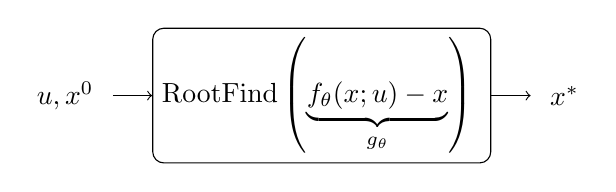
\begin{tikzpicture}[node distance = 0.25cm and 0.5cm, auto, align=center]    
    % blocks
    \node[] (input) {};
    \node[block, right= of input] (G) {
        $\operatorname{RootFind}\left(\underbrace{f_{\theta}(x;u)- x}_{g_{\theta}}\right)$        
    };
    % \node at (G.north) [above] {$\mathcal{S}_{\operatorname{DEQ}}$};
    \node[right= of G] (output) {};
    
    % Input and outputs coordinates
    
    % lines
    \draw[->] (input)  node[left] {$u, x^0$} -- (G);
    \draw[->] (G) -- (output) node[right] {$x^*$} ;    

    

\end{tikzpicture}

\end{document}